\documentclass[12pt]{iopart}
%DIF LATEXDIFF DIFFERENCE FILE
%DIF DEL submission_01.tex   Fri Apr 23 10:06:12 2021
%DIF ADD submission_02.tex   Fri Apr 23 10:42:58 2021

\usepackage{graphicx}
\graphicspath{{../fig/}}

\usepackage{url}
\usepackage{siunitx}
\usepackage{cleveref}
%DIF PREAMBLE EXTENSION ADDED BY LATEXDIFF
%DIF UNDERLINE PREAMBLE %DIF PREAMBLE
\RequirePackage[normalem]{ulem} %DIF PREAMBLE
\RequirePackage{color}\definecolor{RED}{rgb}{1,0,0}\definecolor{BLUE}{rgb}{0,0,1} %DIF PREAMBLE
\providecommand{\DIFadd}[1]{{\protect\color{blue}\uwave{#1}}} %DIF PREAMBLE
\providecommand{\DIFdel}[1]{{\protect\color{red}\sout{#1}}}                      %DIF PREAMBLE
%DIF SAFE PREAMBLE %DIF PREAMBLE
\providecommand{\DIFaddbegin}{} %DIF PREAMBLE
\providecommand{\DIFaddend}{} %DIF PREAMBLE
\providecommand{\DIFdelbegin}{} %DIF PREAMBLE
\providecommand{\DIFdelend}{} %DIF PREAMBLE
\providecommand{\DIFmodbegin}{} %DIF PREAMBLE
\providecommand{\DIFmodend}{} %DIF PREAMBLE
%DIF FLOATSAFE PREAMBLE %DIF PREAMBLE
\providecommand{\DIFaddFL}[1]{\DIFadd{#1}} %DIF PREAMBLE
\providecommand{\DIFdelFL}[1]{\DIFdel{#1}} %DIF PREAMBLE
\providecommand{\DIFaddbeginFL}{} %DIF PREAMBLE
\providecommand{\DIFaddendFL}{} %DIF PREAMBLE
\providecommand{\DIFdelbeginFL}{} %DIF PREAMBLE
\providecommand{\DIFdelendFL}{} %DIF PREAMBLE
\newcommand{\DIFscaledelfig}{0.5}
%DIF HIGHLIGHTGRAPHICS PREAMBLE %DIF PREAMBLE
\RequirePackage{settobox} %DIF PREAMBLE
\RequirePackage{letltxmacro} %DIF PREAMBLE
\newsavebox{\DIFdelgraphicsbox} %DIF PREAMBLE
\newlength{\DIFdelgraphicswidth} %DIF PREAMBLE
\newlength{\DIFdelgraphicsheight} %DIF PREAMBLE
% store original definition of \includegraphics %DIF PREAMBLE
\LetLtxMacro{\DIFOincludegraphics}{\includegraphics} %DIF PREAMBLE
\newcommand{\DIFaddincludegraphics}[2][]{{\color{blue}\fbox{\DIFOincludegraphics[#1]{#2}}}} %DIF PREAMBLE
\newcommand{\DIFdelincludegraphics}[2][]{% %DIF PREAMBLE
\sbox{\DIFdelgraphicsbox}{\DIFOincludegraphics[#1]{#2}}% %DIF PREAMBLE
\settoboxwidth{\DIFdelgraphicswidth}{\DIFdelgraphicsbox} %DIF PREAMBLE
\settoboxtotalheight{\DIFdelgraphicsheight}{\DIFdelgraphicsbox} %DIF PREAMBLE
\scalebox{\DIFscaledelfig}{% %DIF PREAMBLE
\parbox[b]{\DIFdelgraphicswidth}{\usebox{\DIFdelgraphicsbox}\\[-\baselineskip] \rule{\DIFdelgraphicswidth}{0em}}\llap{\resizebox{\DIFdelgraphicswidth}{\DIFdelgraphicsheight}{% %DIF PREAMBLE
\setlength{\unitlength}{\DIFdelgraphicswidth}% %DIF PREAMBLE
\begin{picture}(1,1)% %DIF PREAMBLE
\thicklines\linethickness{2pt} %DIF PREAMBLE
{\color[rgb]{1,0,0}\put(0,0){\framebox(1,1){}}}% %DIF PREAMBLE
{\color[rgb]{1,0,0}\put(0,0){\line( 1,1){1}}}% %DIF PREAMBLE
{\color[rgb]{1,0,0}\put(0,1){\line(1,-1){1}}}% %DIF PREAMBLE
\end{picture}% %DIF PREAMBLE
}\hspace*{3pt}}} %DIF PREAMBLE
} %DIF PREAMBLE
\LetLtxMacro{\DIFOaddbegin}{\DIFaddbegin} %DIF PREAMBLE
\LetLtxMacro{\DIFOaddend}{\DIFaddend} %DIF PREAMBLE
\LetLtxMacro{\DIFOdelbegin}{\DIFdelbegin} %DIF PREAMBLE
\LetLtxMacro{\DIFOdelend}{\DIFdelend} %DIF PREAMBLE
\DeclareRobustCommand{\DIFaddbegin}{\DIFOaddbegin \let\includegraphics\DIFaddincludegraphics} %DIF PREAMBLE
\DeclareRobustCommand{\DIFaddend}{\DIFOaddend \let\includegraphics\DIFOincludegraphics} %DIF PREAMBLE
\DeclareRobustCommand{\DIFdelbegin}{\DIFOdelbegin \let\includegraphics\DIFdelincludegraphics} %DIF PREAMBLE
\DeclareRobustCommand{\DIFdelend}{\DIFOaddend \let\includegraphics\DIFOincludegraphics} %DIF PREAMBLE
\LetLtxMacro{\DIFOaddbeginFL}{\DIFaddbeginFL} %DIF PREAMBLE
\LetLtxMacro{\DIFOaddendFL}{\DIFaddendFL} %DIF PREAMBLE
\LetLtxMacro{\DIFOdelbeginFL}{\DIFdelbeginFL} %DIF PREAMBLE
\LetLtxMacro{\DIFOdelendFL}{\DIFdelendFL} %DIF PREAMBLE
\DeclareRobustCommand{\DIFaddbeginFL}{\DIFOaddbeginFL \let\includegraphics\DIFaddincludegraphics} %DIF PREAMBLE
\DeclareRobustCommand{\DIFaddendFL}{\DIFOaddendFL \let\includegraphics\DIFOincludegraphics} %DIF PREAMBLE
\DeclareRobustCommand{\DIFdelbeginFL}{\DIFOdelbeginFL \let\includegraphics\DIFdelincludegraphics} %DIF PREAMBLE
\DeclareRobustCommand{\DIFdelendFL}{\DIFOaddendFL \let\includegraphics\DIFOincludegraphics} %DIF PREAMBLE
%DIF LISTINGS PREAMBLE %DIF PREAMBLE
\RequirePackage{listings} %DIF PREAMBLE
\RequirePackage{color} %DIF PREAMBLE
\lstdefinelanguage{DIFcode}{ %DIF PREAMBLE
%DIF DIFCODE_UNDERLINE %DIF PREAMBLE
  moredelim=[il][\color{red}\sout]{\%DIF\ <\ }, %DIF PREAMBLE
  moredelim=[il][\color{blue}\uwave]{\%DIF\ >\ } %DIF PREAMBLE
} %DIF PREAMBLE
\lstdefinestyle{DIFverbatimstyle}{ %DIF PREAMBLE
	language=DIFcode, %DIF PREAMBLE
	basicstyle=\ttfamily, %DIF PREAMBLE
	columns=fullflexible, %DIF PREAMBLE
	keepspaces=true %DIF PREAMBLE
} %DIF PREAMBLE
\lstnewenvironment{DIFverbatim}{\lstset{style=DIFverbatimstyle}}{} %DIF PREAMBLE
\lstnewenvironment{DIFverbatim*}{\lstset{style=DIFverbatimstyle,showspaces=true}}{} %DIF PREAMBLE
%DIF END PREAMBLE EXTENSION ADDED BY LATEXDIFF

\begin{document}

\title{How unprecedented was the February 2021 Texas cold snap?}

\author{James Doss-Gollin$^1$, David J. Farnham$^2$, Upmanu Lall,$^{3,4}$ and Vijay Modi$^5$}
\address{$^1$ Department of Civil and Environmental Engineering, Rice University, Houston, TX, USA (ORCID 0000-0002-3428-2224)}
\address{$^2$ Department of Global Ecology, Carnegie Institution for Science, Stanford, CA, USA (ORCID 0000-0002-6690-4251)}
\address{$^3$ Columbia Water Center, Columbia University, New York, NY, USA (ORCID 0000-0003-0529-8128)}
\address{$^4$ Department of Earth and Environmental Engineering, Columbia University, New York, NY, USA}
\address{$^4$ Department of Mechanical Engineering, Columbia University, New York, NY, USA (ORCID 0000-0003-2513-0437)}
\ead{jdossgollin@rice.edu}
\vspace{10pt}

\begin{abstract}
  Winter storm Uri brought severe cold to the southern United States in February 2021, causing a cascading failure of interdependent systems in Texas where infrastructure was not adequately prepared for such cold.
  In particular, the failure of interconnected energy systems reduced electricity supply just as heating demands spiked, leaving millions of Texans without heat or electricity, many for several days.
  This motivates the question: \DIFdelbegin \DIFdel{was the cold }\DIFdelend \DIFaddbegin \DIFadd{were the temperatures }\DIFaddend that contributed to this infrastructure failure \DIFdelbegin \DIFdel{a ``black swan'' that could not have been anticipated}\DIFdelend \DIFaddbegin \DIFadd{beyond what was known to be possible}\DIFaddend , or did historical storms \DIFdelbegin \DIFdel{provide }\DIFdelend \DIFaddbegin \DIFadd{offer }\DIFaddend a precedent?
  We compute the population weighted temperature excursion below \SI{68}{\degree F} as a proxy for heating demand and use this metric to answer the question ``what would the aggregate demand for heating have been had historic cold snaps occurred today?''.
  We find that local temperatures and the inferred demand for heating across the \DIFdelbegin \DIFdel{Texas Interconnect }\DIFdelend \DIFaddbegin \DIFadd{region served by the Texas Interconnection }\DIFaddend during a storm in December 1989 were more \DIFdelbegin \DIFdel{intense }\DIFdelend \DIFaddbegin \DIFadd{severe }\DIFaddend than those recorded during February 2021, and that several other storms in the modern era were comparable.
  Given anticipated population growth, future storms may lead to even greater infrastructure failures if adaptive investments are not made.
  Further, electricity system managers should anticipate that upward trends in electrification of heating may cause peak annual loads on the Texas \DIFdelbegin \DIFdel{Interconnect }\DIFdelend \DIFaddbegin \DIFadd{Interconnection }\DIFaddend to occur during winter storms.

\end{abstract}
\noindent{\it Keywords: Energy, Electricity, Texas, Natural Hazards, Climate Resilience}

\submitto{\ERL}
\maketitle

\section{Introduction}

Between February 14th and 17th, 2021, a northern air mass blanketed much of the continental United States, causing anomalously low surface temperatures across the Great Plains.
While polar air excursions are not unusual, they do not typically reach as far south as the Mexican border.
The state of Texas was particularly hard hit, with coincident and cascading failures of natural gas production, power generation, transportation, and water systems leaving millions of Texans without electricity, heat, and water, many for several days.
The intensity and widespread nature of this weather event underscore a high vulnerability to cold temperatures in places that did not experience a comparable event in preceding decades.
Even as energy demand for winter heating in Texas has grown dramatically with population and economic development, the system’s vulnerability to cold jeopardized lives and property and brought the Texas electricity grid within minutes of collapse.

Since production and distribution of natural gas and electricity is possible under conditions far colder than any Texas experienced in February 2021, energy system failures reflect inadequate preparedness for cold.
If \DIFdelbegin \DIFdel{this were an unprecedented or very rare event }\DIFdelend \DIFaddbegin \DIFadd{these temperatures were unprecedented in the region covered by the Texas Interconnection }\DIFaddend then it is possible that the impacts resulted from an event outside the design envelope.
On the other hand, if similar events were in the record then one would expect a higher level of preparation.
It is therefore important to assess whether \DIFdelbegin \DIFdel{the February 2021 cold snap could have been anticipated.
}\DIFdelend \DIFaddbegin \DIFadd{historical data offered a precedent for the temperatures observed during February 2021.
}\DIFaddend To answer this question, we first compute the population weighted temperature excursion below \SI{68}{\degree F} as a proxy for the unknown heating demand, and use this metric to explore \DIFdelbegin \DIFdel{how rare this event was }\DIFdelend \DIFaddbegin \DIFadd{the frequency with which this event could have been expected to occur }\DIFaddend using historical data.
Next, we conduct a spatially distributed analysis to assess how unexpected the cold experienced by local roads, water mains, gas pipelines, energy generation facilities, and critical infrastructure installations was across Texas.
We conclude by discussing the implications of these findings for long-term electricity systems planning given anticipated population growth and electrification.

\subsection{Previous Cold Snaps in Texas}

It is well documented that Texas has previously experienced severe cold, most notably in 1899, 1951, 1983, 1989, and 2011.
The specific spatiotemporal structure of a cold event, and its correspondence with population centers, modulates the grid-wide demand for heating (\cref{sec:inferred-demand}).
The structure of the storm also drives the aggregated hazard to energy infrastructure, which has implications for the costs and benefits of infrastructure hardening.
It is therefore important to assess the weather conditions that led to these infrastructure failures and identify whether they had historical precedent.

\Cref{fig:historic_era5} and supplemental \cref{fig:historic_bk,fig:historic_tx} show historic cold snaps in Texas.
Although the spatiotemporal structure of each event is distinct, it is apparent that cold extremes in Texas tend to co-occur with cold temperatures across much of the United States, particularly the Great Plains.
While the 2021 event was severe, daily temperature extrema in Texas appear comparable to historical events.
The ``Great Blizzard'' of February 1899, shown in \cref{fig:historic_bk}, caused even more intense cold.

\begin{figure}
  \centering
  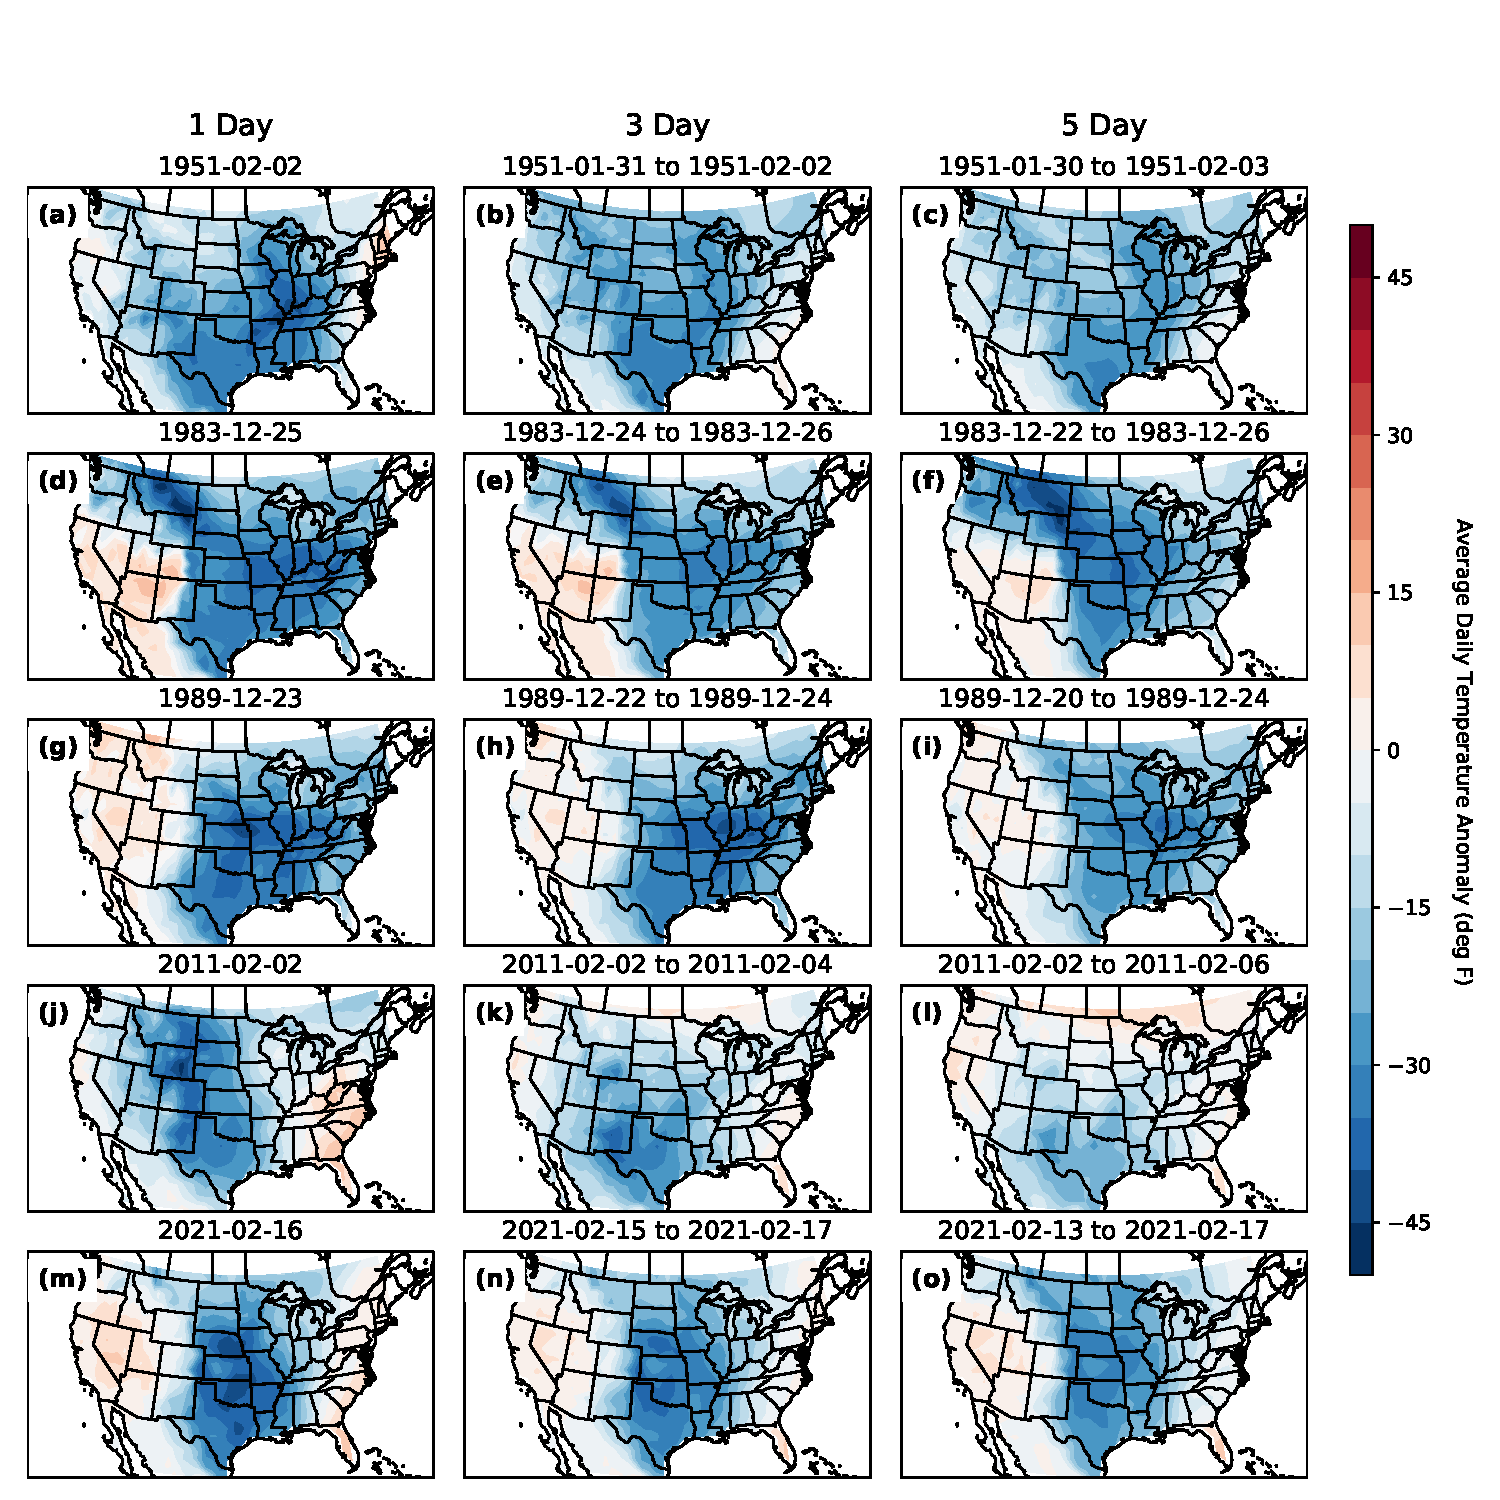
\includegraphics[width=\textwidth]{historic_events_era5.pdf}
  \caption{
    Severe cold snaps that affect Texas and extend into the central United States have several precedents in the historical record.
    Plot shows anomalies of daily mean temperatures for historic major cold events affecting Texas, defined as the departure from the seasonal (December-February) mean to facilitate comparison of events in different calendar months.
    Temperatures over the Continental United States are plotted to show large-scale patterns, but events are selected based only on Texas temperatures.
    Hourly temperatures are averaged to 1-day (a,d,g,j,m), 3-day (b,e,h,k,n), and 5-day (c,f,i,l,o) average temperature anomalies.
  }\label{fig:historic_era5}
\end{figure}

\section{Data and Methods}

We use three distinct datasets to analyze temperature minima in \DIFdelbegin \DIFdel{Texas }\DIFdelend \DIFaddbegin \DIFadd{the region covered by the Texas Interconnection bulk electric power system administered by the Electric Reliability Council of Texas (hence ``Texas Interconnection'') }\DIFaddend through the lens of distributed (each grid cell analyzed separately) and aggregated (weighted averages taken across space) extreme values analysis.

\subsection{Datasets}

We use three temperature datasets to ensure robust findings:
\begin{enumerate}
  \item Hourly \SI{2}{\meter} air temperature reanalysis on a \SI{0.25}{\degree} grid from the ERA-5 reanalysis project produced by the European Centre for Medium Range Weather Forecasting \cite{hersbach_era5:2020} and available  from the Copernicus Data Store (\url{https://cds.climate.copernicus.eu}) from 1950 to the present.
        The period from 1950 to 1979 is released as a preliminary back extension.
        All plots shown in the main text use the ERA-5 data, but supplemental figures use other data sets.
  \item Daily mean, minimum and maximum temperatures, gridded to \SI{1}{\degree}, produced by Berkeley Earth (\url{http://berkeleyearth.org/data/}).
        This gridded product is based on statistical analysis of station data and is available from 1880 to 2019.
        This dataset is considered an experimental product, so we use it only for comparative purposes.
  \item To complement blended gridded data products, we use station temperature data from the Global Historical Climatology Network (GHCN) dataset compiled by the National Ocean and Atmospheric Administration \cite{Menne:2012hk} and available at \url{https://www1.ncdc.noaa.gov/pub/data/ghcn/daily/}.
        This dataset provides daily mean, maximum, and minimum temperature observations.
        These measurements represent point measurements, which can differ in important ways from gridded products describing spatial averages due to the spatial heterogeneity of temperature fields.
        We retain stations within the state of Texas if they provide at least 60 years of data and if they contain observations for the set of historical cold extremes shown in \cref{fig:historic_era5}.
\end{enumerate}
We also use population density data from the GPWv4 dataset \cite{ciesin_gpwv4:2016}, a list of power generation facilities from the US Energy Information Administration \cite{useia_generators:2021}, and a map of the Texas \DIFdelbegin \DIFdel{Interconnect \mbox{%DIFAUXCMD
    \cite{useia_regions:2021}}\hspace{0pt}%DIFAUXCMD
  .}\DIFdelend \DIFaddbegin \DIFadd{Interconnection \mbox{%DIFAUXCMD
    \cite{useia_regions:2021}}\hspace{0pt}%DIFAUXCMD
  .%DIF > TODO: add and cite information on the generators that did and did not go out.
}\DIFaddend


\subsection{Inferred \DIFaddbegin \DIFadd{per Capita }\DIFaddend Demand for Heating}\label{sec:inferred-demand}

Most space heating in Texas is either electric or gas \cite{waite_heating:2020} and the majority of power generation in the Texas \DIFdelbegin \DIFdel{Interconnect }\DIFdelend \DIFaddbegin \DIFadd{Interconnection }\DIFaddend depends on natural gas \cite{everhart_iea:2021}.
Stress on natural gas production and delivery was therefore just as important as the more visible stress on the electric system.

The hourly or daily thermal energy requirement for space heating is primarily driven by how much lower the ambient temperature is than an indoor comfort temperature of \SI{68}{\degree F}.
This relationship is often expressed in terms of heating degree days or hours.
We therefore consider the temperature excursion from \SI{68}{\degree F} as a proxy for thermal heating demand.
We compute this value each hour for the ERA5 data, defining heating demand at each grid cell as $\text{HD}_t = \max (68 - T_t, 0)$, where $T_t$ is the temperature at hour $t$ in \si{\degree F}.
The Berkeley Earth and GHCN datasets provide daily minimum and maximum temperatures, so we define heating demand at each grid cell or station as $\text{HD}_d = \max (68 -\frac{T_{\text{min},d} + T_{\text{max},d}}{2}, 0)$, where $T_{\text{min},d}$ is the minimum temperature recorded on day $d$ and $T_{\text{max},d}$ is the maximum temperature recorded on day $d$, both in \si{\degree F}.

To assess how spatially correlated cold spells might affect the Texas electric grid, we average heating demand in space over the Texas \DIFdelbegin \DIFdel{Interconnect }\DIFdelend \DIFaddbegin \DIFadd{Interconnection }\DIFaddend domain \cite{useia_regions:2021}, weighting each grid cell by 2020 population density \cite{ciesin_gpwv4:2016}.
We refer to this spatially aggregated time series, which has the straightforward interpretation as the average heating demand experienced by Texas residents, as ``Inferred \DIFaddbegin \DIFadd{per Capita }\DIFaddend Demand for Heating.''

\subsection{Return Period}

For each event duration considered, return periods are obtained by fitting a stationary generalized extreme value (GEV) distribution to the time series of annual minimum December-February (DJF) temperatures, or to the time series of annual maxima of inferred \DIFaddbegin \DIFadd{per capita }\DIFaddend demand for heating (\cref{sec:inferred-demand}).
Events that occur in December are coded to the following year.
The 2021 winter season was excluded from return period estimates, allowing us to interpret return periods for the February 2021 event as \emph{a priori} estimates.

\subsection{Cold Duration}

The effect of cold temperatures on energy demand and critical infrastructure depends on how long the cold persists.
Short duration cold snaps can kill plants, freeze exposed pipes, freeze wind turbines, and contribute to dangerous roadway conditions.
Longer duration cold spells contribute to demand for heating and energy and cause pipes to burst even if they have some insulation.
We calculate demand for heating by taking temporal averages over a range of durations from 1 hour to 4 days.

\subsection{Code and Data}

We are committed to open science.
Our open source code is freely available in a live repository at \url{https://github.com/jdossgollin/2021-TXtreme} and in an archived repository at \url{https://dx.doi.org/10.5281/zenodo.4568923}.
Reproducibility is facilitated through the Snakemake library \cite{koster_snakemake:2012}.

\section{How extreme was inferred \DIFaddbegin \DIFadd{per capita }\DIFaddend heating demand over the Texas Interconnect?}

The total shock to Texas heating demand is partially determined by the extent to which cold snaps impact multiple population centers simultaneously.
As such, understanding whether there was precedent for a cold snap simultaneously affecting several regions of Texas's grid that today have high population density is critical.
We therefore use our measure of inferred \DIFaddbegin \DIFadd{per capita }\DIFaddend demand for heating (see \cref{sec:inferred-demand}) to represent the aggregate heating demand induced by cold temperatures.
Aggregating historic temperature fields in space using the 2020 population, we answer the question ``what would the aggregate demand for heating have been had historic cold snaps occurred today?''

\Cref{fig:idf_weighted} shows that the intensity, duration, and recurrence intervals of the February 2021 storm are severe but not unprecedented in the historical record.
For example, at the 6 hour duration the December 1989 storm was substantially more intense and other storms including February 1951 were nearly as intense.
At the two day duration, the 2021 and 1989 events were approximately equally intense and other storms including December 1983 were nearly as intense.
The 2011 storm, which caused rolling blackouts and motivated research into the energy system's vulnerability to cold \cite{ferc_outages:2011}, was quite modest by comparison.
The right panel shows statistical return periods for these extreme events\DIFdelbegin \DIFdel{, though these estimates are sensitive to small changes in inferred demand for heating}\DIFdelend .

\begin{figure}
  \centering
  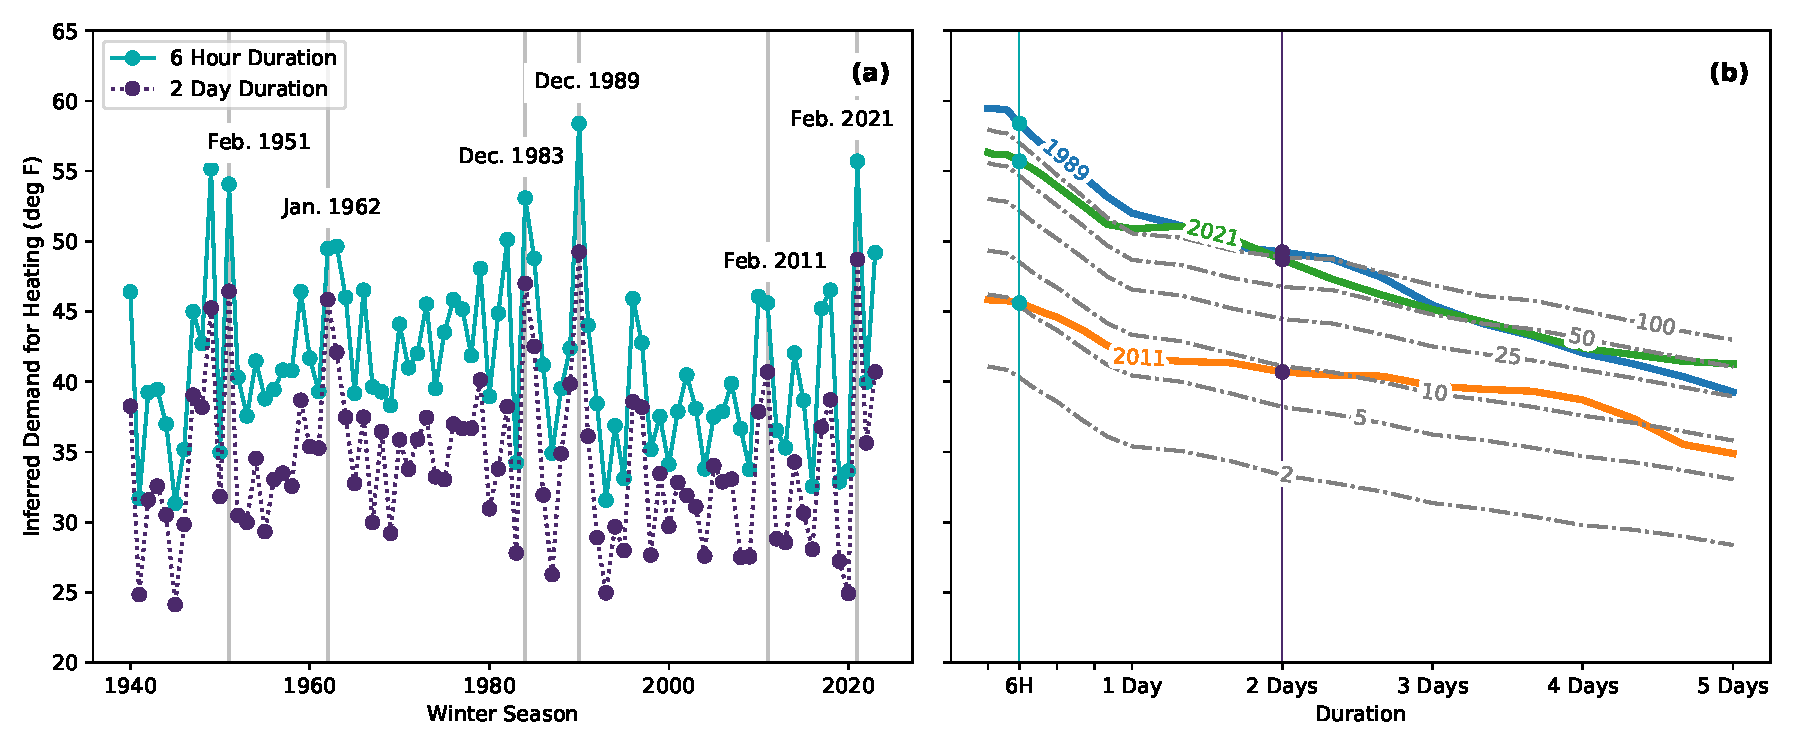
\includegraphics[width=\textwidth]{ERCOT_HDD_IDF_MLE_popweighted.pdf}
  \caption{
    The inferred \DIFaddbeginFL \DIFaddFL{per capita }\DIFaddendFL demand for heating induced by the February 2021 cold snap is not unprecedented.
    For the worst 6 hours, the 1989 event was more severe than the 2021 event, while they are comparable for the longer durations.
    (a): time series of annual maximum inferred \DIFaddbeginFL \DIFaddFL{per capita }\DIFaddendFL demand for heating (\cref{sec:inferred-demand}) at 6 hour and 2 day durations.
    December extremes, including the December 1989 storm, are coded to the following year so that one maximum per December-February winter season is taken.
    (b): the intensity-duration-frequency intervals estimated using 1950-2020 data (i.e., not using the 2021 event), overlaid by the annual maxima from the 1989, 2011, and 2021 events.
    Gray dashed lines indicate 2, 5, 10, 25, 50, and 100 year return levels.
  }\label{fig:idf_weighted}
\end{figure}

\section{Spatially distributed temperature extremes}

It is difficult to establish a spatially aggregated proxy for supply-side risk given complex interlinkages between natural gas, electric, and other systems which create the possibility for cascading failures as observed in February 2021.
Water treatment and distribution systems, as well as other essential services, also rely on electricity, further increasing vulnerabilities.
Instead of aggregating this risk in space, we estimate the exceedance probability of the February 2021 temperatures at each grid cell separately to shed light on the severity of cold experienced by installations across the region.

\Cref{fig:local_era5} shows local return periods for the February 2021 cold snap at 6 hour, 1 day, 2 day, and 4 day durations.
Other than a band from south-central to south-east Texas, nearly all regions of the Texas \DIFdelbegin \DIFdel{Interconnect }\DIFdelend \DIFaddbegin \DIFadd{Interconnection }\DIFaddend (gray outline in \cref{fig:local_era5}a,d) experienced cold with a return period below 50 years.
Results are similar using station data (\cref{fig:local_ghcnd}).
Importantly for the energy system, the band experiencing cold with return period greater than 50 years includes a substantial fraction of Texas’s population (\cref{fig:local_era5}a) and natural gas generation (\cref{fig:local_era5}d).
Outside the Texas \DIFdelbegin \DIFdel{Interconnect }\DIFdelend \DIFaddbegin \DIFadd{Interconnection }\DIFaddend region, much of the Texas Panhandle and central Oklahoma experienced intense cold with a return period greater than 100 years at multiple durations.
Although Oklahoma recorded some water main breaks \cite{crum_water:2021} and rolling blackouts for several hours \cite{money_oklahoma:2021}, infrastructure impacts were less severe than in Texas despite recording more extreme (relative both to its own historical record and in absolute terms) temperatures.

\begin{figure}
  \centering
  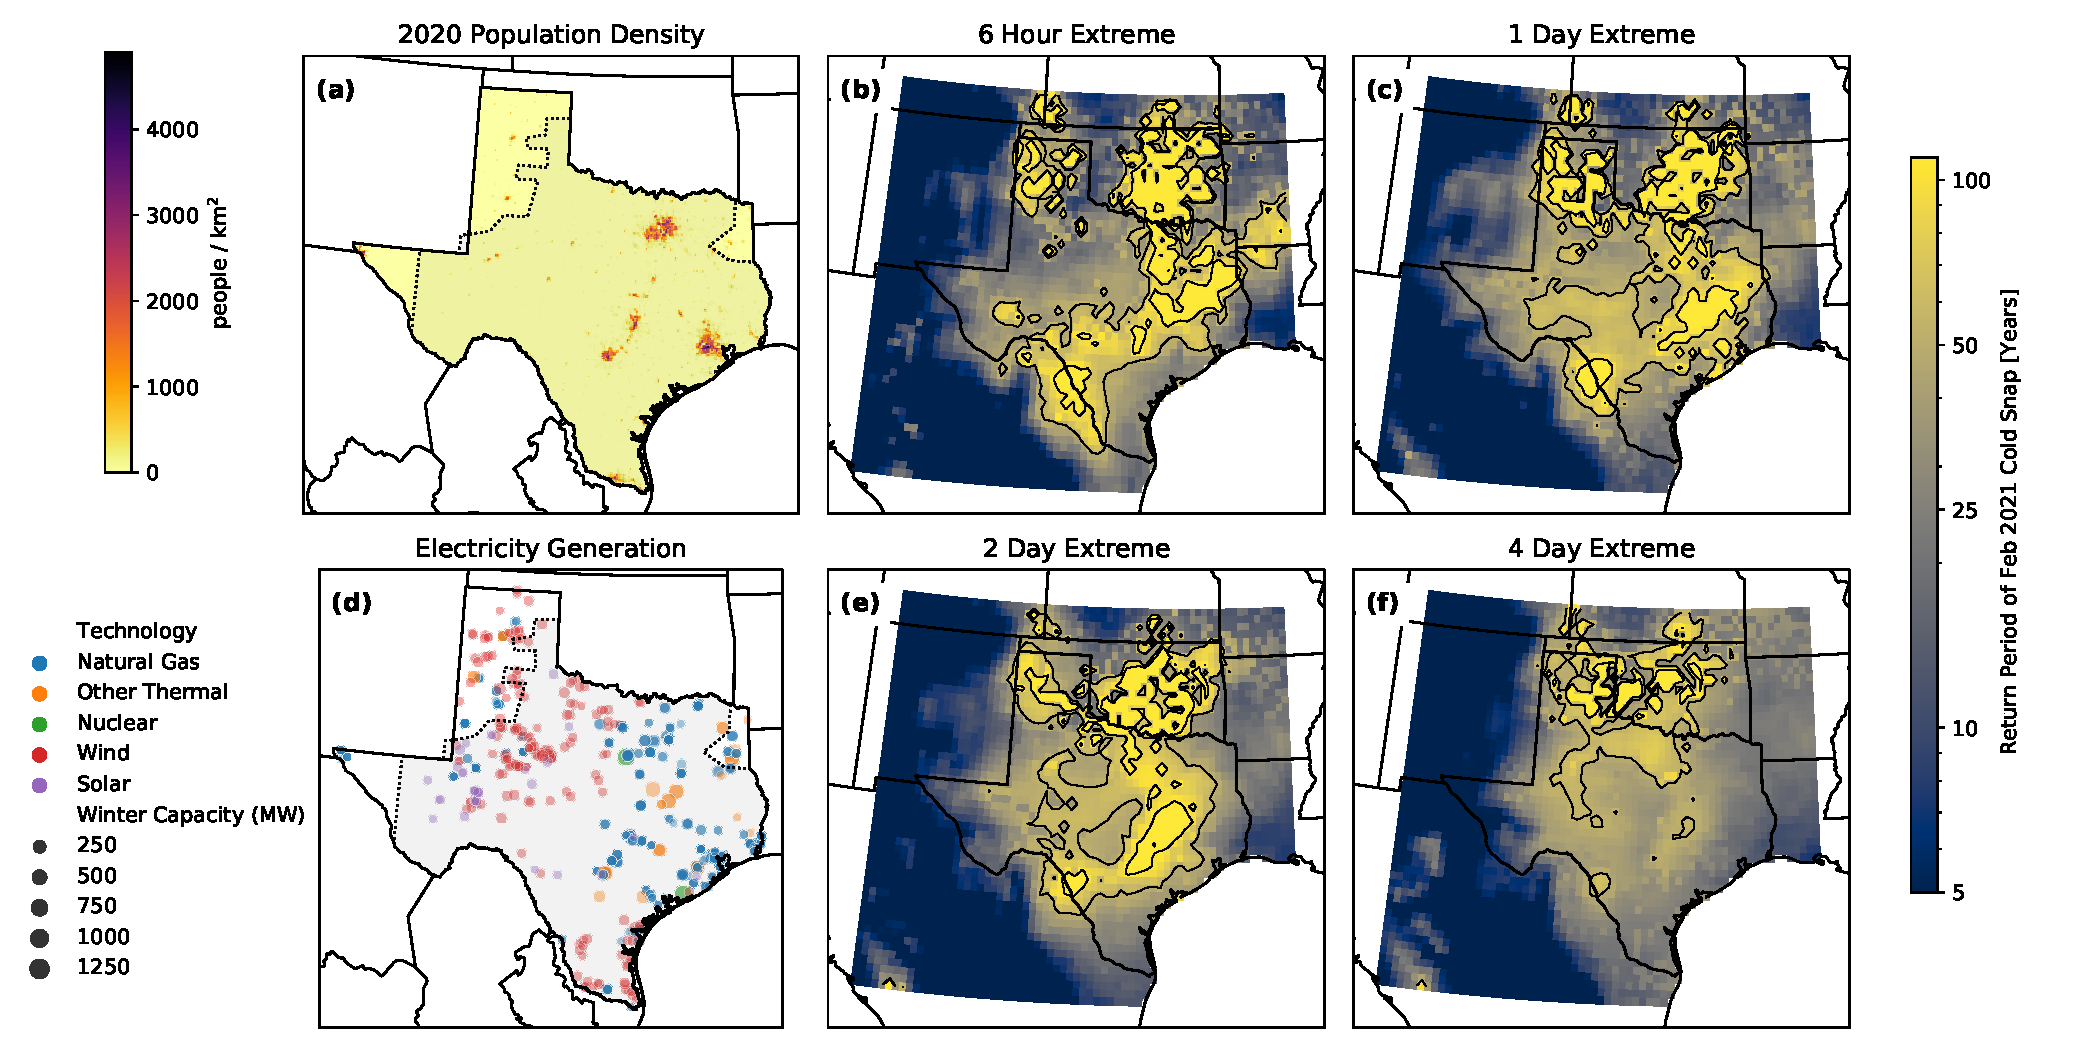
\includegraphics[width=\textwidth]{local_rt_era5.pdf}
  \caption{
    Return periods for the February 2021 event, calculated using stationary estimates of annual extremes over the period 1950-2020.
    Return periods are calculated separately for each cell.
    (a): estimates of 2020 population density \cite{ciesin_gpwv4:2016}.
    (d): energy generation facilities in Texas \cite{useia_generators:2021}.
    (b,c,e,f): local return periods for 6 hour, 1 day, 2 day, and 4 day durations, respectively.
    Contours enclose regions that recorded 50 and 100 year return levels.
    The gray region in panels (a) and (d) shows boundaries of the Texas \DIFdelbeginFL \DIFdelFL{Interconnect }\DIFdelendFL \DIFaddbeginFL \DIFaddFL{Interconnection }\DIFaddendFL \cite{useia_regions:2021}.
  }\label{fig:local_era5}
\end{figure}

\section{Discussion}

Our spatially aggregated metric of inferred \DIFaddbegin \DIFadd{per capita }\DIFaddend demand for heating shows that the February 2021 event was intense but not unforeseeable (\cref{fig:idf_weighted}).
Although specific locations experienced very intense ($>100$ year return period) temperatures, we find that for most locations in Texas the temperatures recorded during the February 2021 cold snap had precedent in the historical record\DIFdelbegin \DIFdel{and could have been anticipated given available data}\DIFdelend .

A proximate cause of load shedding in the Texas \DIFdelbegin \DIFdel{Interconnect }\DIFdelend \DIFaddbegin \DIFadd{Interconnection }\DIFaddend during February 2021 was the vulnerability of the electricity generation system to the severe cold temperatures \cite{everhart_iea:2021}.
\Cref{fig:local_era5,fig:local_ghcnd} show that this happened even though most parts of the state had previously experienced similarly intense cold, notably in 1989.
While our analysis neglects other meteorological factors, like freezing rain, that may have impeded operations at specific facilities, our analysis suggests that the February 2021 failures of energy and electricity systems in the Texas \DIFdelbegin \DIFdel{Interconnect }\DIFdelend \DIFaddbegin \DIFadd{Interconnection }\DIFaddend took place during temperatures comparable to those previously recorded.
Similarly, water mains broke in places like Houston where temperatures did not exceed 100-year return levels, underscoring characteristic vulnerability of critical infrastructure systems \cite{chester_reliable:2020}.

Another cause of load shedding was the high demand for electricity that low temperatures induced.
Currently over 50\% of Texas households use electricity for space heating over the majority of census tracts of the state \cite{waite_heating:2020} and further electrification is a central element of many plans to decarbonize our energy sector \cite{williams_decarbonization:2012,davis:2018,white_txresidential:2019}.
While summer peak loads have been a central planning concern on the Texas grid in the past, it is likely that winter peak loads will become a greater concern in the coming decades.
In fact, the peak demand during this event was estimated at around \SI{74.5}{\giga\watt}, just shy of the all time peak for any season of \SI{74.8}{\giga\watt} in August 2019 \cite{everhart_iea:2021}.
As electrification of heating increases, severe cold snaps may represent the peak demand on the Texas Interconnect.

Our primary findings hold for an alternative gridded dataset and station data (see supplemental material).
However, calculated return periods are sensitive to the method of estimation (\cref{fig:idf_lmoments_unweighted,fig:idf_lmoments_weighted}).
Future analysis could address parametric uncertainty, model structure uncertainty \cite{wong_floodrisk:2018}, non-stationarity \cite{Milly:2008dg}, or regime-like modes of climate variability \cite{DossGollin:2019}.
More fundamentally, an assessment of exposure to cold extremes over the next decades should consider the deeply uncertain distribution of future climate change, and the induced effect on cold extremes in Texas.
Although a broad scientific consensus suggests the frequency of cold extremes should decrease under warming in most places \cite{ipcc_ar5:2014}, possible links between North-South temperature gradients and mid-latitude temperature extremes remains an area of active research \cite{Barnes:2013fp,Cohen:2014gx,Screen:2013ho}.
Regardless, the effect of climate change on peak demand for heating is likely to be small compared to the effect of rapid population growth; for example, the Texas Water Development Board anticipates at least 40\% growth from 2020 to 2050 \cite{texaswaterplan:2012}.

Our analysis quantifies the \DIFdelbegin \DIFdel{probability with which temperature extremes }\DIFdelend \DIFaddbegin \DIFadd{frequency with which the temperatures observed during February 2021 }\DIFaddend could have been \DIFdelbegin \DIFdel{anticipated }\DIFdelend \DIFaddbegin \DIFadd{expected to occur }\DIFaddend \emph{a priori}.
Other factors also govern infrastructure performance and failure, including precipitation, the demand for natural gas in adjacent regions, and complex connections within and between regional systems.
Similarly, decisions at multiple time scales, including disaster preparedness and risk communication, contribute to the human consequences of physical infrastructure failure.
Thus, the exact chain of events that led to the blackouts and water system disruptions during February 2021 should be sorted out only after thorough investigations by parties on the ground in Texas.

\section{Conclusions}

The February 2021 cold snap was the most intense in 30 years, but was not without precedent in the full historical record.
In addition to the record cold conditions of 1899 (\cref{fig:historic_bk}), we estimate that the weather of December 1989 would have resulted in slightly higher 6-hour and 2-day aggregate heating demands over the Texas \DIFdelbegin \DIFdel{Interconnect }\DIFdelend \DIFaddbegin \DIFadd{Interconnection }\DIFaddend had it occurred in February 2021.
Several other storms since 1950 would have produced nearly as much demand for heating.
Given upward trends in the electrification of heating, it is likely that future cold snaps will cause peak annual loads on the Texas \DIFdelbegin \DIFdel{Interconnect }\DIFdelend \DIFaddbegin \DIFadd{Interconnection }\DIFaddend to occur during the winter season.
Infrastructure expansion necessitated by a rapidly growing population offers Texas the opportunity to invest in a more resilient energy system.

\section*{Acknowledgements}

DJF was supported by a gift from Gates Ventures LLC to the Carnegie Institution for Science.
The authors thank
Sylvia Dee,
Elisabeth Gawthrop,
Adam Massmann,
and
Vivek Srikrishnan
for comments on a preliminary draft of this manuscript.
The authors also thank the developers and maintainers of the open source packages we used, in particular the pydata and pangeo communities, and the many journalists and academics whose timely reporting and commentary has informed our thinking.

\section*{Bibliography}
\bibliographystyle{unsrt}
\bibliography{references}

\clearpage
\appendix
\section{Supplemental Results}
\renewcommand{\thefigure}{S\arabic{figure}}
\setcounter{figure}{0}

\subsection{Historic Extreme Temperatures}

To complement \cref{fig:historic_era5}, we plot extreme cold temperatures using alternate data.
First, \cref{fig:historic_bk} shows historic events over the Continental United States.
The set of events is slightly different than that of \cref{fig:historic_era5}: the data set does not include the 2021 event, but does include the 1899 ``Great Blizzard.''
The 1899 event shows more intense and persistent cold than the other events in the dataset.
Next, \cref{fig:historic_tx} shows the same data as \cref{fig:historic_era5} but zooms in on Texas.
The 1989 (g-i) and 2021 (m-o) appear to be the most severe events in this data set, and the 1-day cold extremes in the 1989 event are more intense than in the February 2021 event, consistent with results in the main text.

\begin{figure}
  \centering
  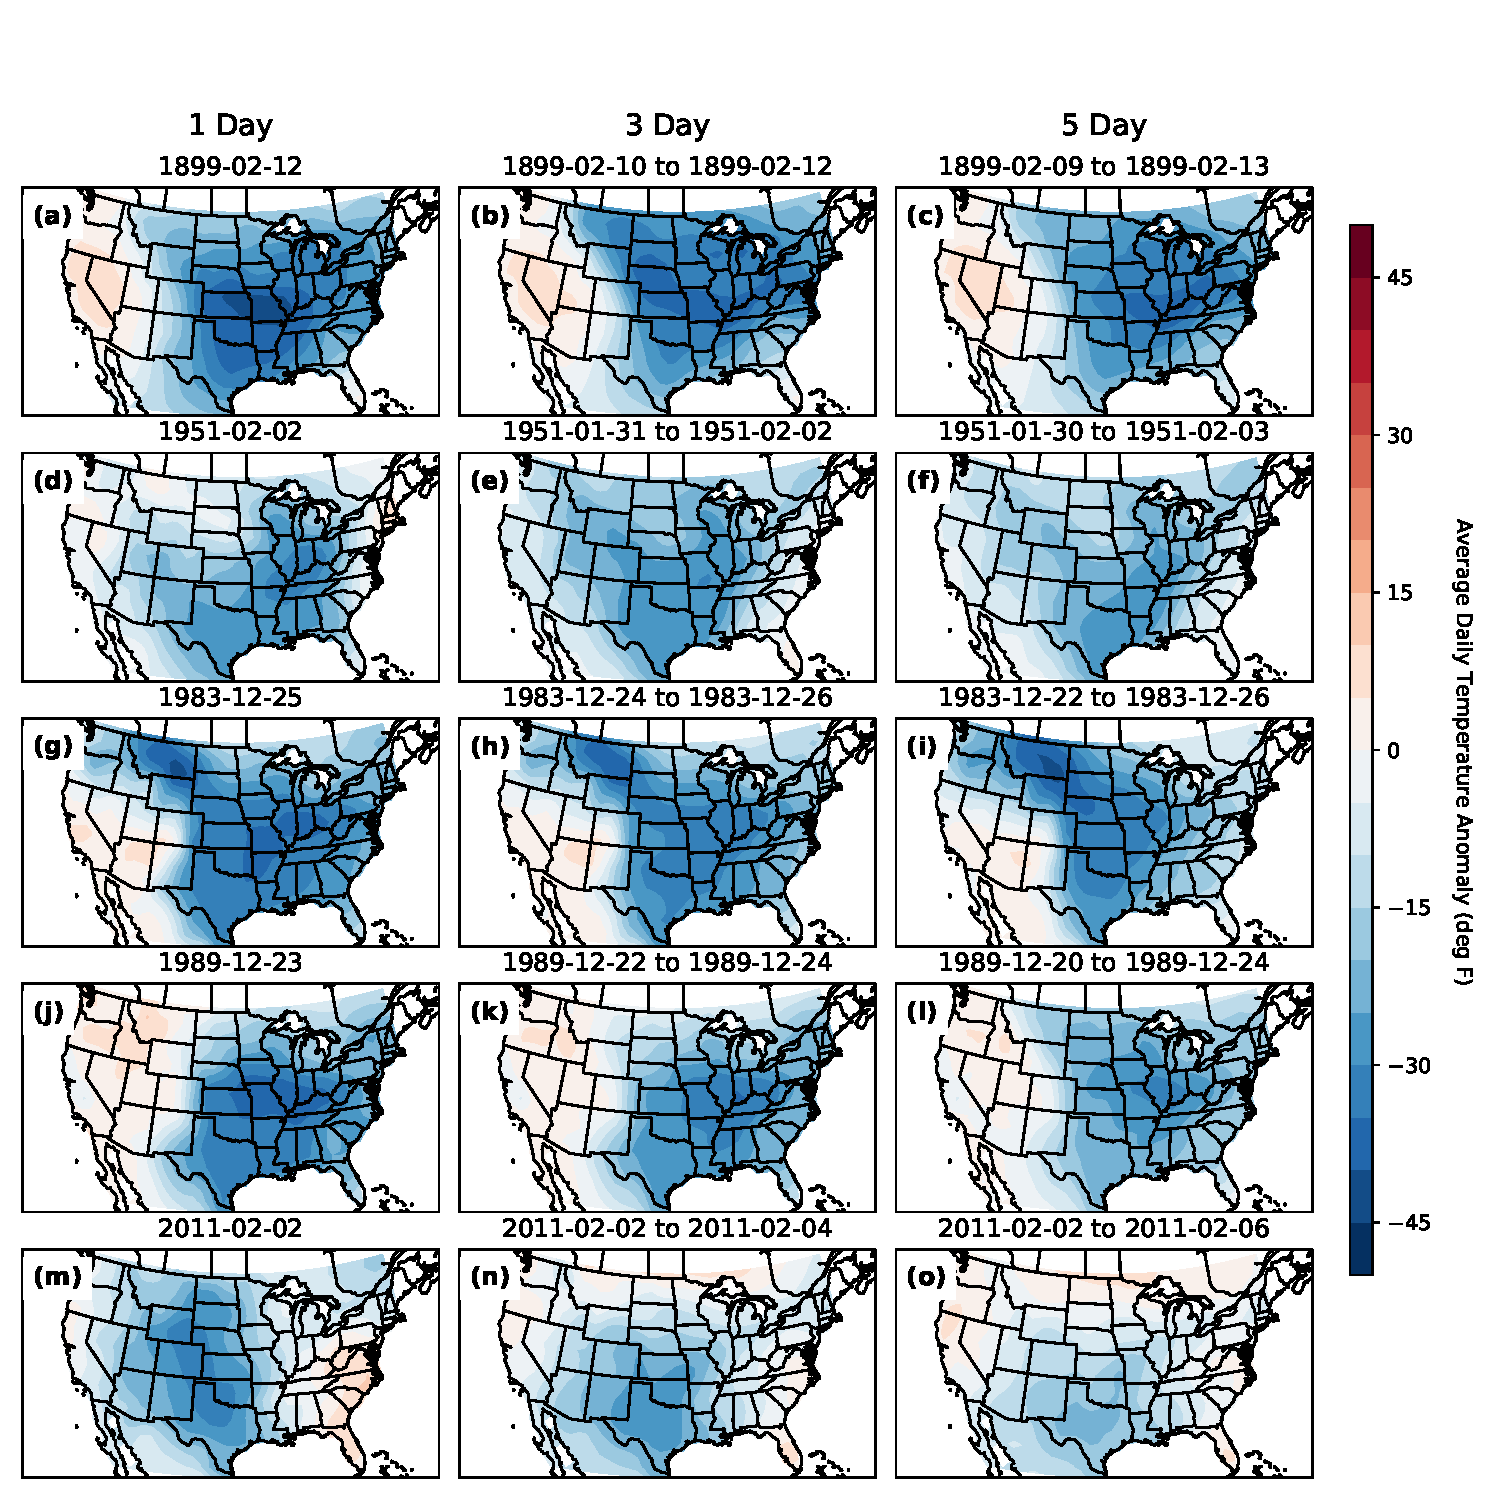
\includegraphics[width=\textwidth]{historic_events_bk.pdf}
  \caption{
    As \cref{fig:historic_bk} but the Berkely Earth temperature data is used.
    The dataset does not contain the 2021 event, but the ``Great Blizzard'' of February 1899 is included.
    Spatial patterns of cold from this dataset are qualitatively similar to Figure 1.
    The 1899 event emphasizes that the modern historical record does not yield a full sample from the full distribution of possible hazards.
  }\label{fig:historic_bk}
\end{figure}

\begin{figure}
  \centering
  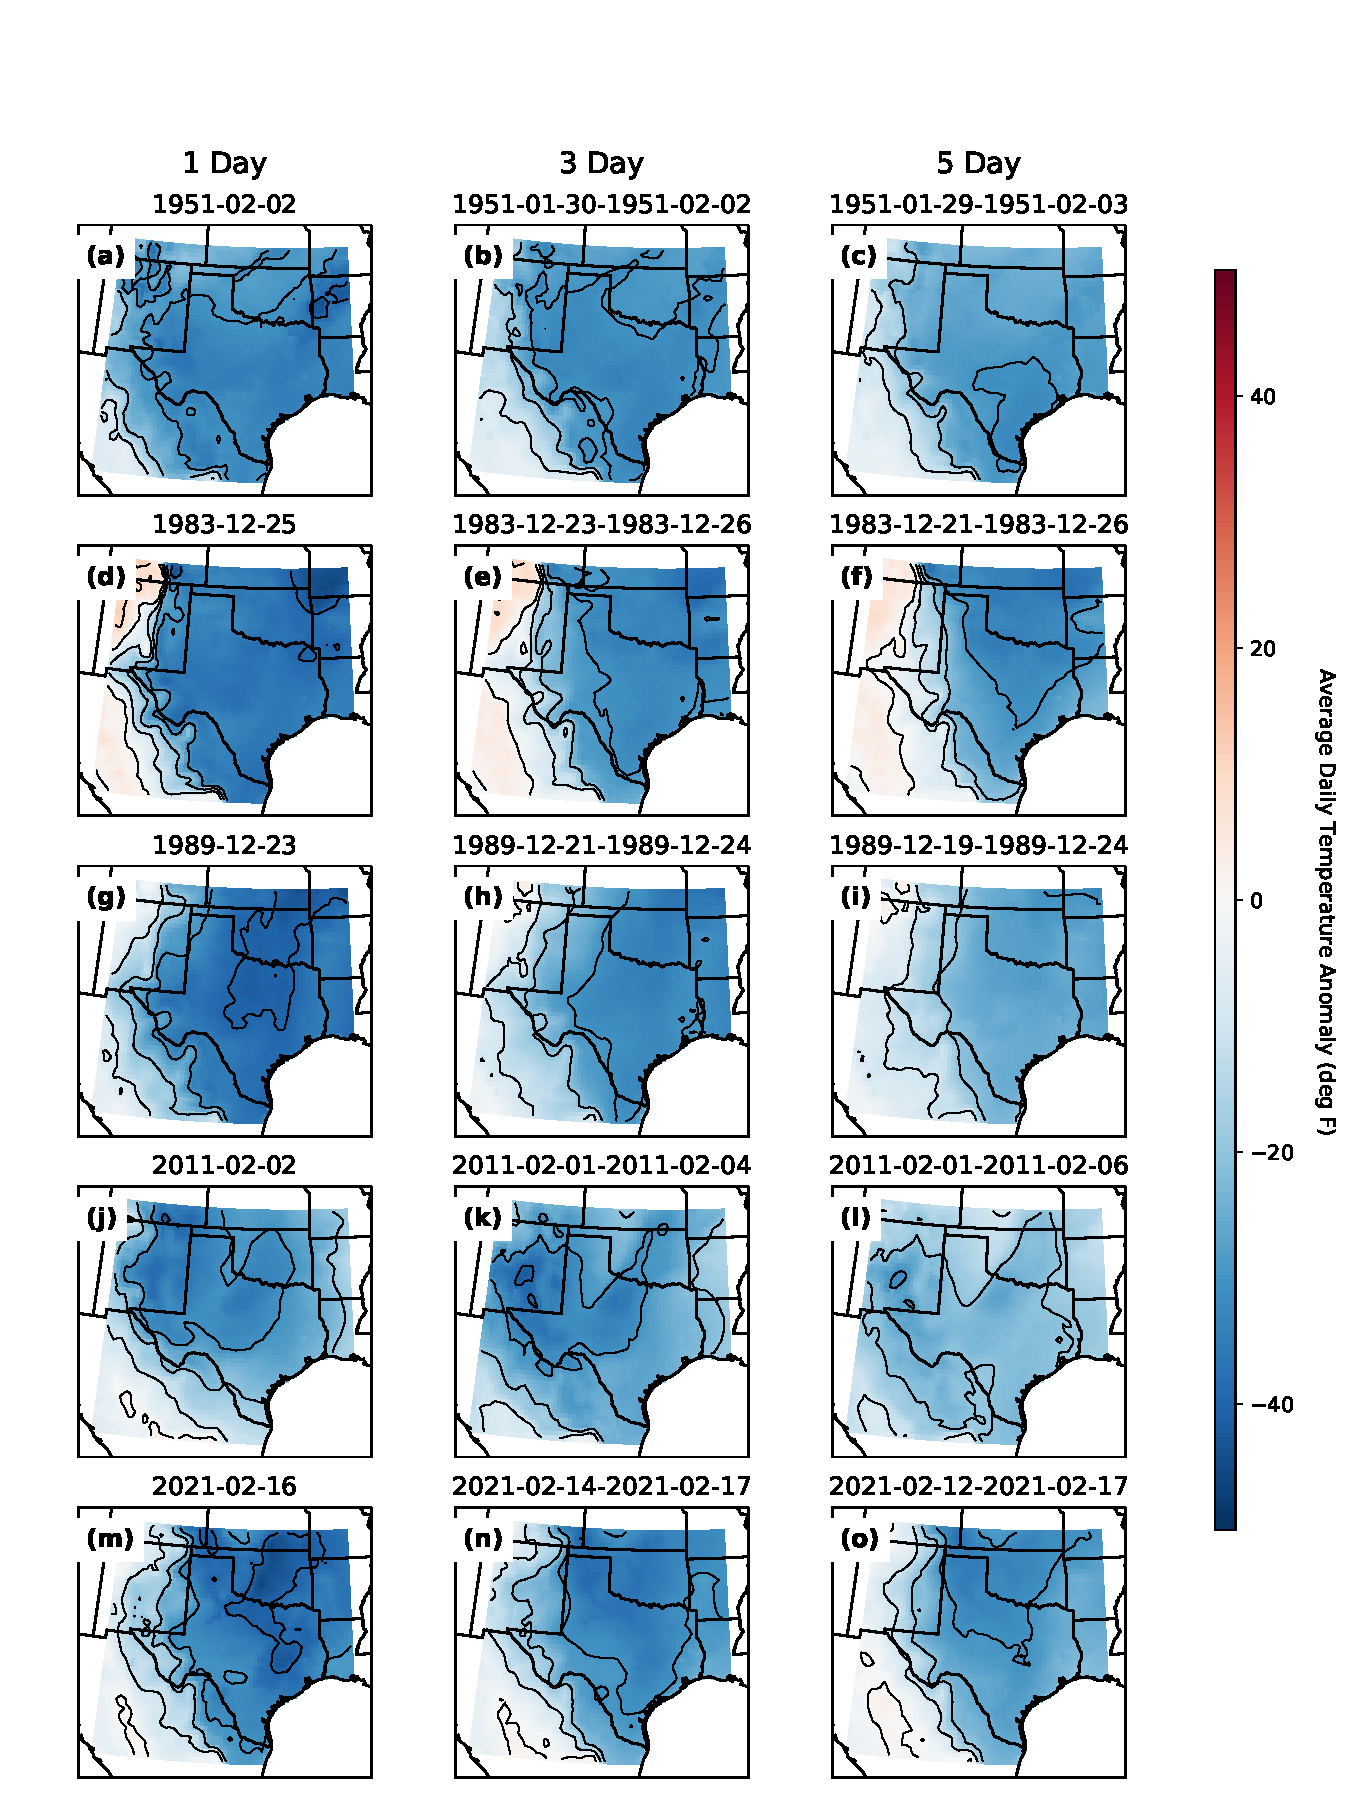
\includegraphics[width=\textwidth]{historic_events_era5_TX.pdf}
  \caption{
    As \cref{fig:historic_bk} but only Texas is shown.
  }\label{fig:historic_tx}
\end{figure}

\subsection{Spatially distributed temperature extremes}

To complement \cref{fig:local_era5}, we compute local return periods using station data from the GHCN \cite{Menne:2012hk}.
\Cref{fig:local_ghcnd} shows the return periods of the February 2021 cold snap for 1, 2, 3, and 4 day durations.
Only stations with at least 60 years of data are considered, and since the locations of these stations are not chosen at random, this does not constitute a representative sample of all points across Texas.
However, the spatial pattern matches that of \cref{fig:local_era5}, with a band of severe cold stretching from south-central to eastern Texas and in the Texas Panhandle.

\subsection{Inferred \DIFaddbegin \DIFadd{per capita }\DIFaddend demand for heating}

To complement our analysis of inferred \DIFaddbegin \DIFadd{per capita }\DIFaddend demand for heating, we consider how results change as a function of two modeling decisions.
First, we consider what happens if the spatial field demand for heating is aggregated using grid cell area rather than population density.
Next, we compute return periods using an estimator based on the method of $L$-moments.
Although $L$-moment estimators for the generalized extreme value distribution are not unbiased, they are popular in the statistical hydrology literature for their stability \cite{hosking_gev:1985,martins_gev:2001,morrison_gev:2002}.

We draw two conclusions from these plots.
First, the 2021 event appears more severe if grid cells are weighted by population density (\cref{fig:idf_weighted,fig:idf_lmoments_weighted}) than if they are weighted only by area \cref{fig:idf_unweighted,fig:idf_lmoments_unweighted}).
This is consistent with our observation of a correspondence between the most extreme temperatures in February 2021 and population density (\cref{fig:local_era5}).
By contrast, the 2011 event appears more extreme when grid cells are weighted by area, which is consistent with \cref{fig:historic_tx,fig:historic_era5,fig:historic_bk} showing the coldest temperatures in relatively less populated West Texas.
Second, the $L$-moment estimators (\cref{fig:idf_lmoments_weighted,fig:idf_lmoments_unweighted}) assign a lower return period to the 1989 and 2021 events than the maximum likelihood estimators (\cref{fig:idf_unweighted,fig:idf_weighted}).

To provide some context for our inferred demand for heating metric, \cref{fig:hdd_ts} plots its time series during the peak of the February 2021 cold snap.
This reveals a rise from approximately \SI{10}{\degree F} to nearly \SI{60}{\degree F} during the peak of the February 2021 cold snap.

\begin{figure}
  \centering
  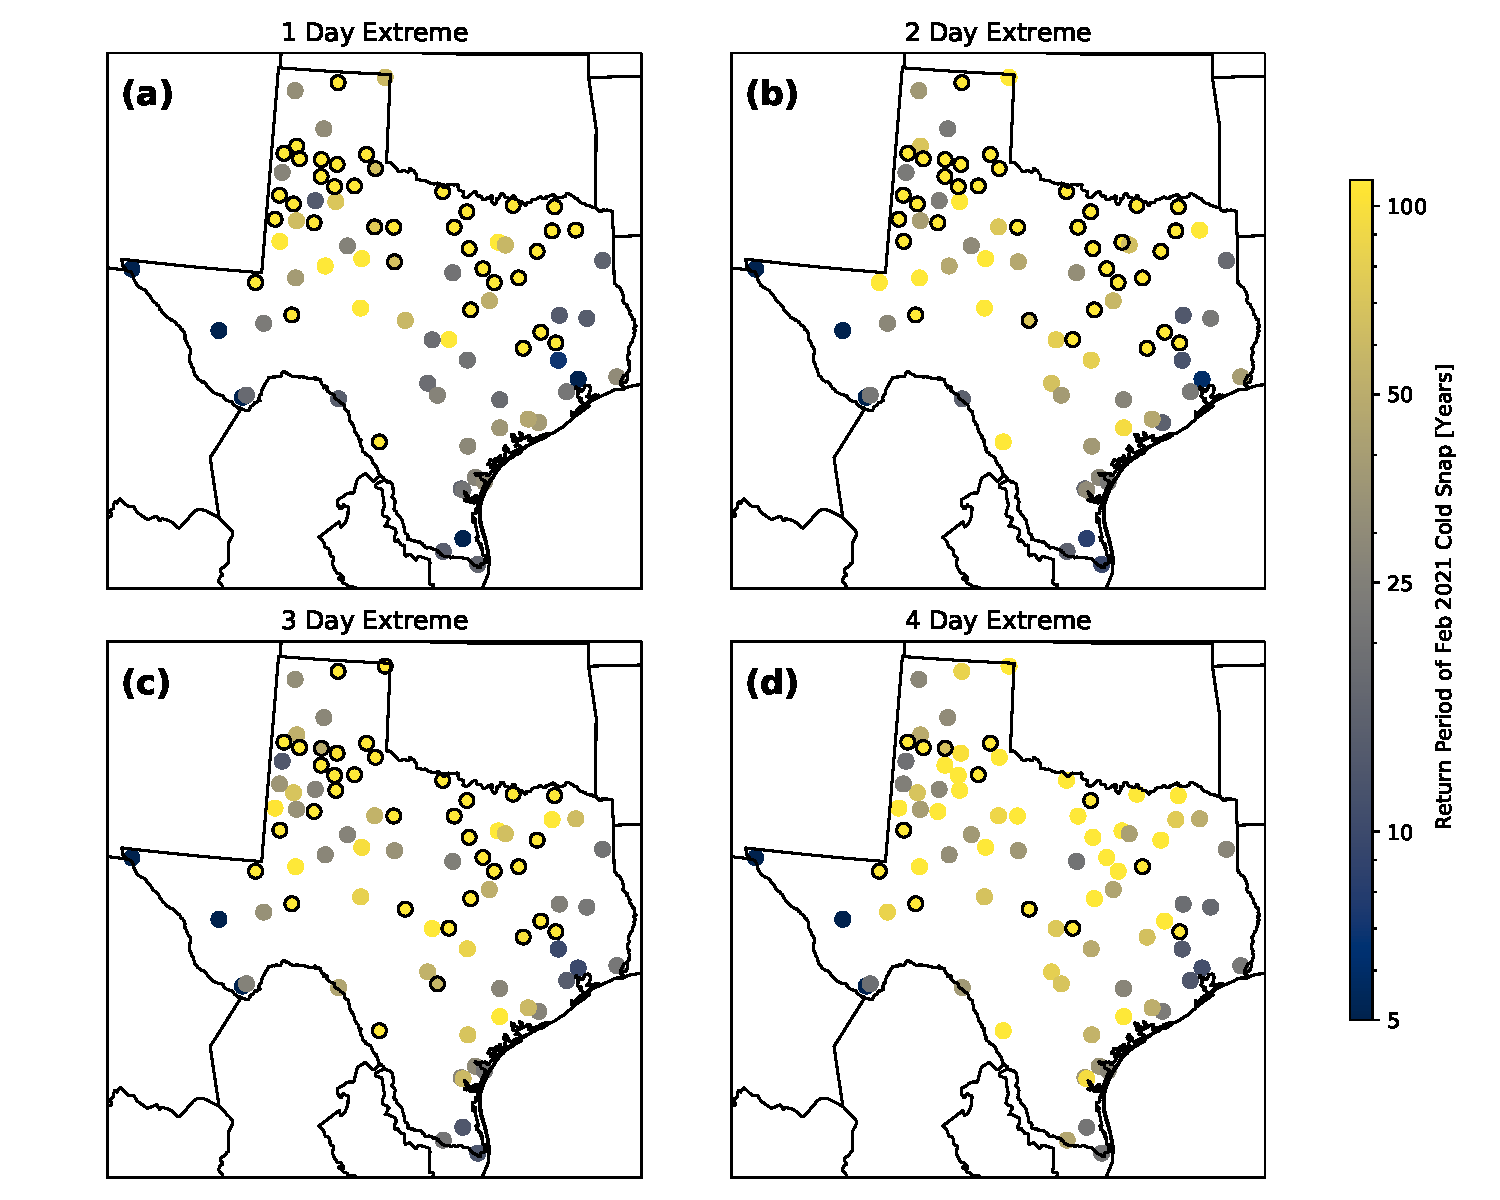
\includegraphics[width=\textwidth]{local_rt_ghcnd.pdf}
  \caption{
    As \cref{fig:local_era5} but return periods are calculated using station data from the GHCN data set \cite{Menne:2012hk}.
    Black circles indicate that a station exceeded its own record for a particular duration.
  }\label{fig:local_ghcnd}
\end{figure}

\begin{figure}
  \centering
  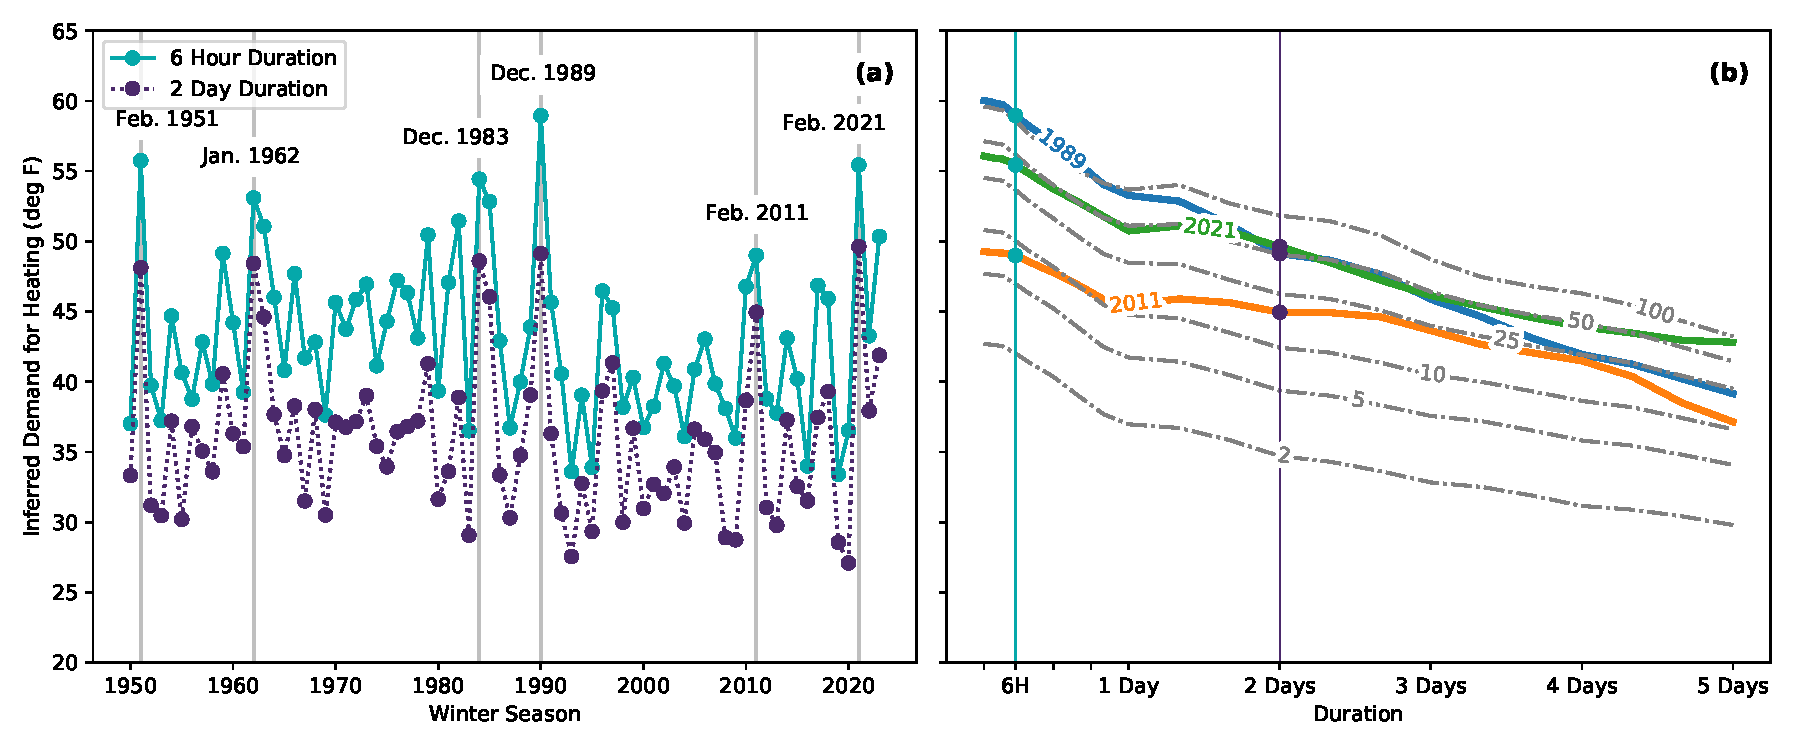
\includegraphics[width=\textwidth]{ERCOT_HDD_IDF_MLE_unweighted.pdf}
  \caption{
    As \cref{fig:idf_unweighted} but grid cells are weighted by area $A=\cos(\phi)$ where $\phi$ is latitude.
  }\label{fig:idf_unweighted}
\end{figure}

\begin{figure}
  \centering
  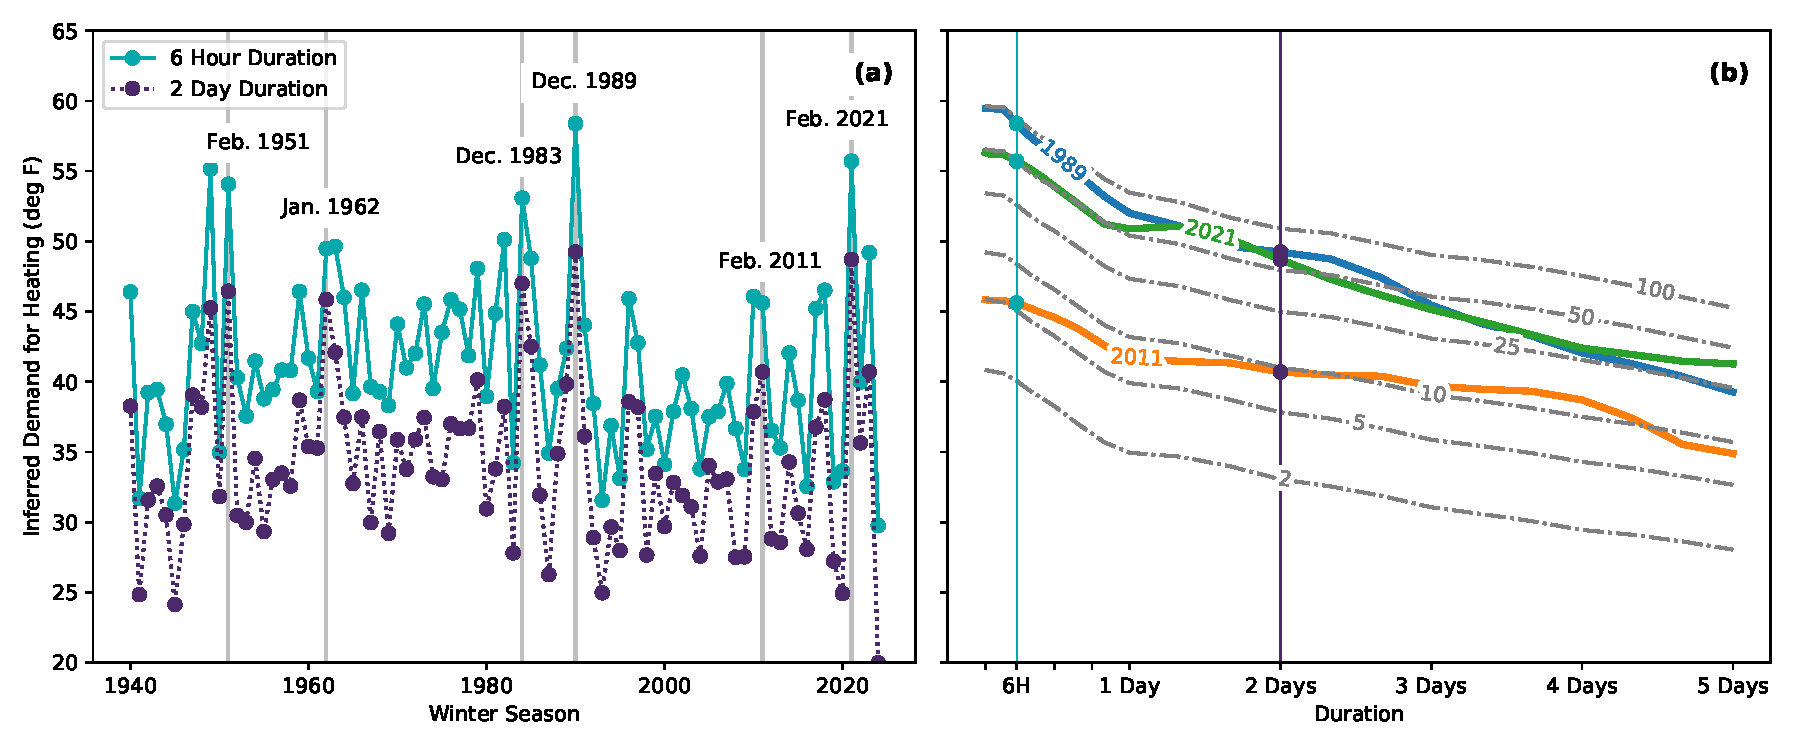
\includegraphics[width=\textwidth]{ERCOT_HDD_IDF_plotpos_popweighted.pdf}
  \caption{
    As \cref{fig:idf_unweighted} but return periods are calculated using the $L$-moments estimator.
  }\label{fig:idf_lmoments_weighted}
\end{figure}

\begin{figure}
  \centering
  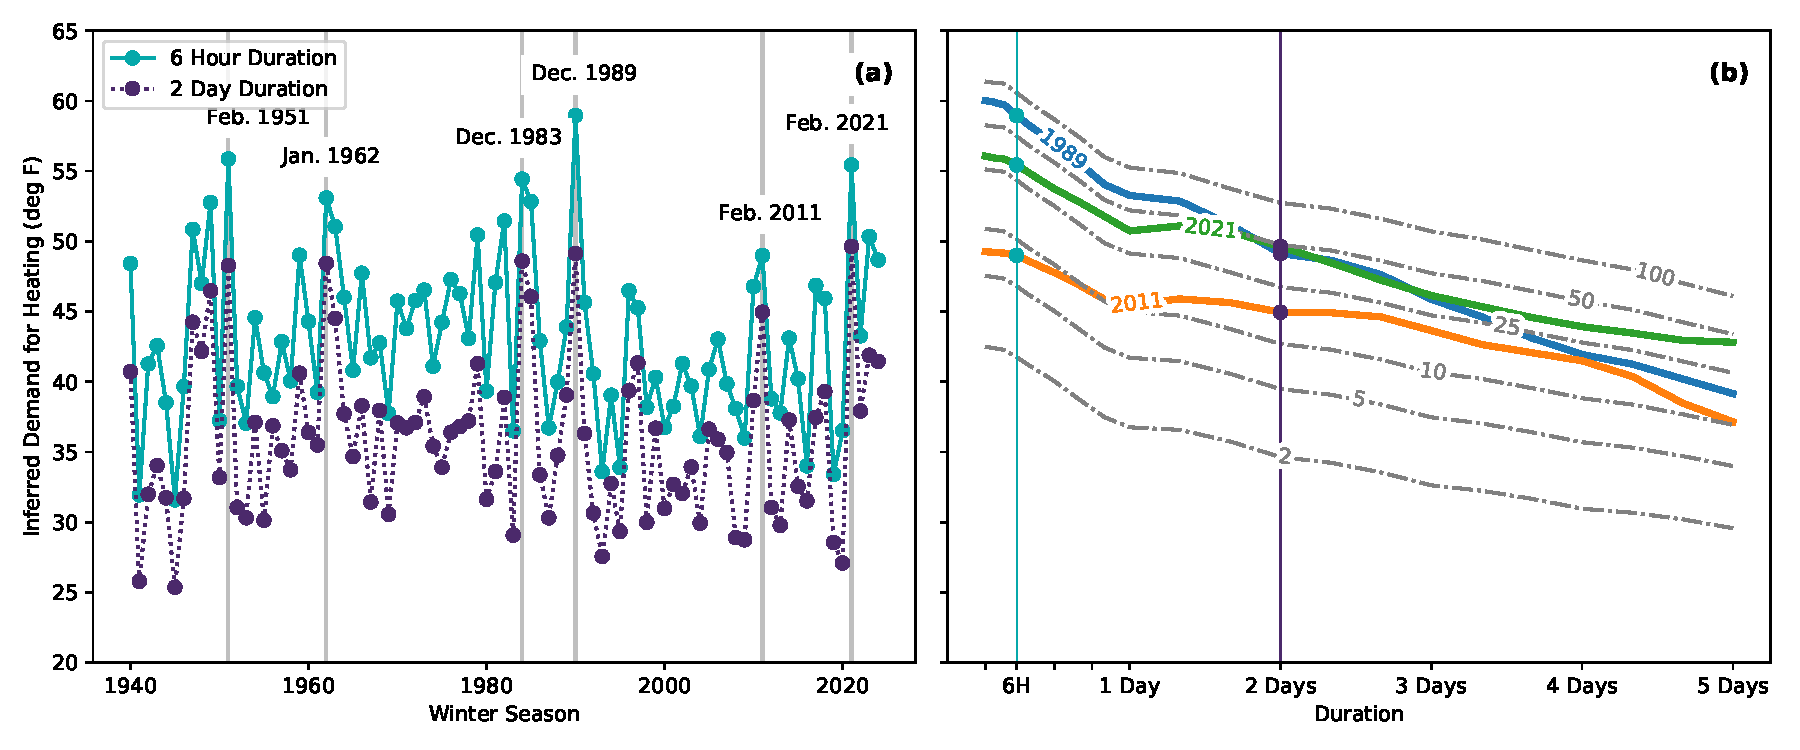
\includegraphics[width=\textwidth]{ERCOT_HDD_IDF_plotpos_unweighted.pdf}
  \caption{
    As \cref{fig:idf_unweighted} but return periods are calculated using the $L$-moments estimator.
  }\label{fig:idf_lmoments_unweighted}
\end{figure}

\begin{figure}
  \centering
  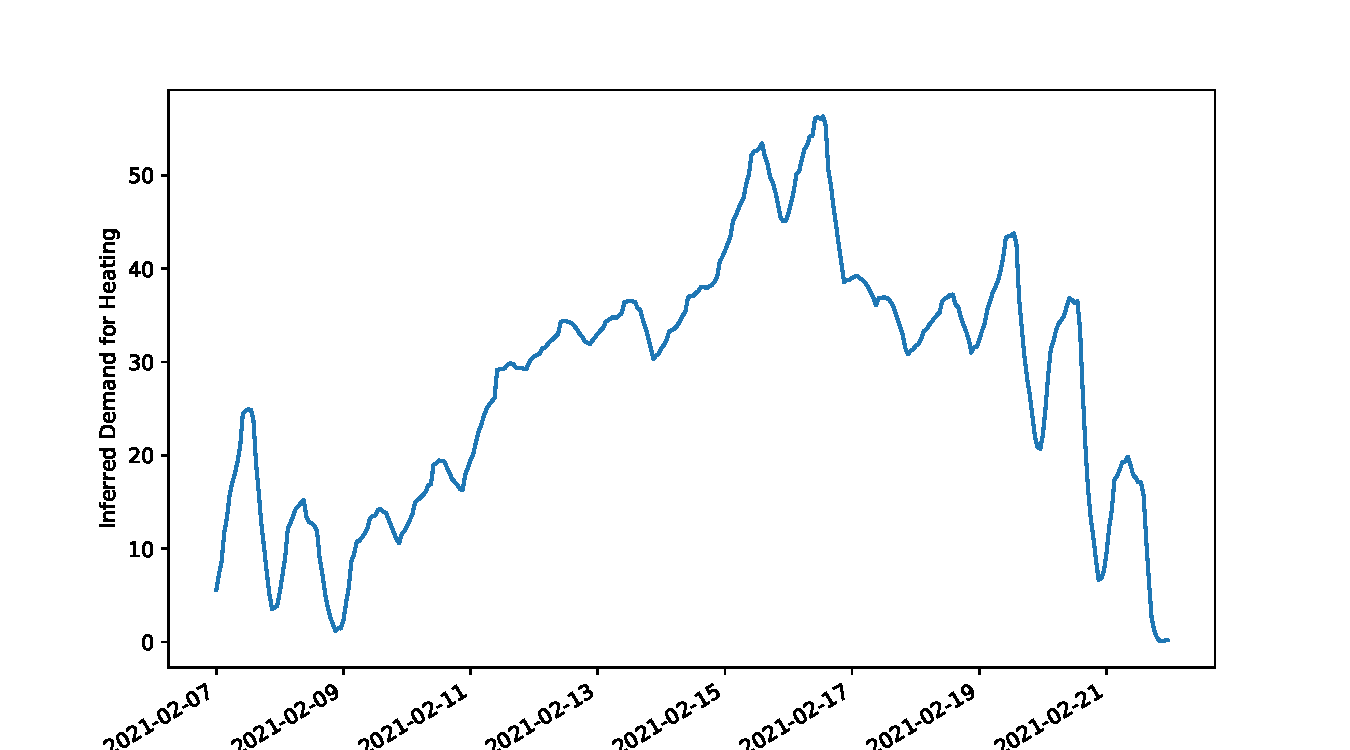
\includegraphics[width=\textwidth]{HDD_pop_weighted_ts.pdf}
  \caption{
    A time series of inferred \DIFaddbeginFL \DIFaddFL{per capita }\DIFaddendFL demand for heating over the Texas \DIFdelbeginFL \DIFdelFL{Interconnect }\DIFdelendFL \DIFaddbeginFL \DIFaddFL{Interconnection }\DIFaddendFL during the February 2021 cold snap.
  }\label{fig:hdd_ts}
\end{figure}

\end{document}

